%%%%%%%%%%%%
%
% $Autor: Wings $
% $Datum: 2019-03-05 08:03:15Z $
% $Pfad: ArduinoIDE.tex $
% $Version: 4250 $
% !TeX spellcheck = en_GB/de_DE
% !TeX encoding = utf8
% !TeX root = filename 
% !TeX TXS-program:bibliography = txs:///biber
%
%%%%%%%%%%%%


\chapter{PlatformIO IDE}


	Dieses Kapitel führt in die Nutzung der PlatformIO-Umgebung innerhalb von Visual Studio Code ein. Es beschreibt den Installationsprozess von PlatformIO in \ac{vscode}, erläutert die grundlegende Struktur eines PlatformIO-Projekts sowie die Konfiguration für das Board Arduino MKR WAN 1310. Darüber hinaus wird gezeigt, wie externe Bibliotheken über das PlatformIO-Registry gesucht, installiert und in ein Projekt eingebunden werden. Schrittweise Anleitungen und Abbildungen unterstützen den praktischen Einstieg in die Embedded-Entwicklung mit PlatformIO.


    
\section{Übersicht über PlatformIO}
	
	\HREF{https://platformio.org}{PlatformIO} ist ein plattformübergreifendes, architekturunabhängiges und mehrframeworkfähiges Tool für Embedded-System-Ingenieure und Softwareentwickler, die Anwendungen für eingebettete Systeme schreiben.
	
	Es handelt sich um eine Open-Source-Software, die die Arbeit mit verschiedenen Prozessoren, Boards, Frameworks und Umgebungen wie Arduino oder ESP-IDF ermöglicht. Sie ist für Windows, Linux, macOS sowie andere kleine ARM-basierte Rechner verfügbar. Entwickelt mithilfe von Python, unterstützt sie C und C++.
	
	Neben der Nutzung innerhalb einer IDE kann sie auch als eigenständiges Kommandozeilenprogramm (\HREF{https://docs.platformio.org/en/latest/core/index.html}{PlatformIO Core}) verwendet werden.
	
	Das Tool ist mit zahlreichen Entwicklungsumgebungen wie Atom, Eclipse, Emacs, NetBeans, Vim und Visual Studio kompatibel. Die bevorzugte Wahl ist jedoch \acl{vscode}, dessen Oberfläche in diesem Zusammenhang oft einfach als PlatformIO bezeichnet wird \cite{PlatformIO:2025}.

	
	
	PlatformIO Projekt aus drei zentralen Komponenten:
	
	\begin{itemize}
		\item Editor - zum Schreiben und Bearbeiten des Codes
		\item Compiler - zur Übersetzung in Maschinencode und Übertragung auf das Entwicklungsboard
		\item \href{https://docs.platformio.org/en/latest/projectconf/index.html}{\FILE{platformio.ini}} - Datei – zur Konfiguration des Mikrocontrollers, verwendeter Bibliotheken und weiterer wichtiger Parameter wie Board-Typ oder Kommunikationsgeschwindigkeit
	\end{itemize}


	\begin{center}
		
\includegraphics[width=0.7\linewidth]{PlatformIO/PlatformIOMenu}
		\captionof{figure}{Menu Buttons}
	\end{center}
	

\section{Installation von PlatformIO für \ac{vscode}}\label{sec:PlatformIOInstallation}

	Im bereits installierten \ac{vscode} wird die Erweiterungssuche geöffnet und nach ,,PlatformIO'' gesucht. Der Downloadvorgang beginnt nach dem Anklicken der Schaltfläche \textit{Install}. Dabei ist darauf zu achten, dass die neueste Version installiert wird.
	
	\begin{center}
		
\includegraphics[width=0.7\linewidth]{PlatformIO/PlatformIODownload}
		\captionof{figure}{Erweiterungssuche in \ac{vscode}}
		\label{fig:PlatformIODownload}
	\end{center}
	
	Nach dem Herunterladen der PlatformIO - \ac{ide} sollte \ac{vscode} neu gestartet werden. Nach dem erneuten Öffnen sollte ein neues PlatformIO-Symbol in der Seitenleiste erscheinen.
	
	\begin{center}
		
\includegraphics[width=0.7\linewidth]{PlatformIO/PlatformIOIcon}
		\captionof{figure}{Menu Buttons}
		\label{fig:PlatformIOIcon}
	\end{center}
	
	Jetzt klicken wir auf das neue Symbol und dann im ,,Quick Access'' unter PIO Home auf ,,Open''. Daraufhin erscheint die folgende Ansicht:
	
	\begin{center}
		
\includegraphics[width=0.7\linewidth]{PlatformIO/PlatformIOView}
		\captionof{figure}{Menu Buttons}
		\label{fig:PlatformIOView}
	\end{center}
	
	

\section{Bibliotheken hinzufügen}

	Externe Bibliotheken sind ein wichtiger Bestandteil jedes Projekts. PlatformIO verfügt über einen gro{\ss}en Pool an Bibliotheken, die sich leicht in ein PlatformIO-Projekt integrieren lassen. Die Bibliotheken können im \href{https://registry.platformio.org}{PlatformIO Registry} gefunden werden.

	\subsection{Bibliothek suchen}
	Um die benötigte Bibliothek zu finden, ist der Name in das Suchfeld einzugeben. Anschlie{\ss}end erscheint eine Liste mit passenden Ergebnissen. Die für das Projekt relevante Position ist auszuwählen:
	
	\begin{center}
		\begin{tikzpicture}
			% obrazek jako tło
			\node[anchor=south west, inner sep=0] (image) at (0,0) {%
				
\includegraphics[width=0.7\linewidth]{PlatformIO/AddBib/PIOFindLib}};
			
			\begin{scope}[x={(image.south east)}, y={(image.north west)}]
				% fastLED Search Place
				\draw[red, line width=4pt, ->, >=angle 60] (0.43,0.9) -- (0.26,0.96);
				\draw[red, line width=2pt] (0.17,0.94) rectangle ++(0.08, 0.05);
				
				% fastled: position on the list
				\draw[red, line width=3pt, <-, >=angle 60] (0.56,0.545) -- ++(0.2,0);
				\draw[red, line width=2pt] (0.32,0.52) rectangle ++(0.22, 0.06);
			\end{scope}
		\end{tikzpicture}
		\captionof{figure}{Beispielsuche: FastLED-Bibliothek}
		\label{fig:PIOFindLib}
	\end{center}
	
	
	\subsection{Bibliothek ins Projekt hinzufügen}
	Nach dem Öffnen einer Position sind in der Regel mehrere Reiter sichtbar. Neben \PYTHON{README.md} ist insbesondere der Reiter \textit{Installation} relevant, da er Informationen darüber liefert, wie eine Bibliothek in das Projekt eingebunden werden muss.
	
	Nach der Auswahl des Reiters \textit{Installation} werden Implementierungsmöglichkeiten angezeigt:
	
	\begin{center}
		\begin{tikzpicture}
			% obrazek jako tło
			\node[anchor=south west, inner sep=0] (image) at (0,0) {%
				
\includegraphics[width=0.7\linewidth]{PlatformIO/AddBib/PIOImplementLib}};
			
			\begin{scope}[x={(image.south east)}, y={(image.north west)}]
				\draw[red, line width=4pt, <-, >=angle 60] (0.37,0.755) -- ++(0.2,-0.1);
				
				% lib_deps
				\draw[red, line width=2pt] (0.06,0.52) rectangle ++(0.5, 0.08);
				
				% #include <XXXX.h>
				\draw[red, line width=2pt] (0.06,0.32) rectangle ++(0.35, 0.08);
	
			\end{scope}
		\end{tikzpicture}
		\captionof{figure}{Ansicht des Installationsreiters}
		\label{fig:PIOImplementLib}
	\end{center}
	
	
	Wie zu sehen ist, muss im Fall der Bibliothek \textit{FastLED} die Position \PYTHON{fastled/FastLED@\^3.10.2} in die Datei \FILE{platformio.ini} eingetragen werden:
	
	\begin{center}
		\begin{tikzpicture}
		% obrazek jako tło
		\node[anchor=south west, inner sep=0] (image) at (0,0) {%
			
\includegraphics[width=0.7\linewidth]{PlatformIO/AddBib/PIOLibPosInPlatformioini}};
		
			\begin{scope}[x={(image.south east)}, y={(image.north west)}]
				\draw[red, line width=4pt, <-, >=angle 60] (0.205,0.310) -- ++(0.1,-0.2);
				
				\draw[red, line width=2pt] (0.4,0.01) rectangle ++(0.35, 0.23);
				
			\end{scope}
		\end{tikzpicture}
		\captionof{figure}{Eintrag der Bibliothek in \texttt{platformio.ini}}
		\label{fig:PIOLibPosInPlatformioini}
	\end{center}
	
	Um die Bibliothek verwenden zu können, darf das Header-File \PYTHON{\#include <FastLED.h>} nicht vergessen werden:
	
	\begin{center}
		\begin{tikzpicture}
			% obrazek jako tło
			\node[anchor=south west, inner sep=0] (image) at (0,0) {%
				
\includegraphics[width=0.7\linewidth]{PlatformIO/AddBib/PIOLinIncludeIntoFile}};
			
			\begin{scope}[x={(image.south east)}, y={(image.north west)}]
				\draw[red, line width=4pt, <-, >=angle 60] (0.215,0.05) -- ++(0.1, 0.2);
				
				\draw[red, line width=2pt] (0.47,0.6) rectangle ++(0.25, 0.08);
				
			\end{scope}
		\end{tikzpicture}
		\captionof{figure}{Einbindung der Bibliothek in den Quellcode}
		\label{fig:PIOLinIncludeIntoFile}
	\end{center}
	
	Die Bibliothek und ihre fehlenden Abhängigkeiten werden bei der Kompilierung des Projekts automatisch heruntergeladen
	
\section{Übertragen des Hello-Blink-Beispiels}
	Im Folgenden wird gezeigt, wie ein erstes Beispielprogramm auf das Board übertragen wird. Das Hello-Blink-Programm dient als einfaches Demonstrationsbeispiel für den Upload eines Projekts sowie für die grundlegende Funktionalität der seriellen Kommunikation und der integrierten Status-LED.
	
	Der Code in \autoref{code:HelloBlink} gibt jede Sekunde die Meldung \textit{Hello - LED Blink} im seriellen Monitor aus und schaltet die integrierte LED im Sekundentakt ein und aus.
	
	{
		\captionof{code}{Hello-Blink-Beispiel für den Arduino MKR WAN 1310}
		\label{code:HelloBlink}
		\ArduinoExternal{}{../../Code/MKRWAN1310/PlatformIO/HelloBlink.cpp}
	}
	
	Der Upload und die Ausführung des Programms erfolgen anhand der folgenden Schritte:
	
	\begin{enumerate}
		\item Übertragen des Codes auf das Arduino-Board
		
		Um den Code zu übertragen, wird der Pfeil \textit{Upload} angeklickt. Anschlie{\ss}end beginnt die Kompilierung und Übertragung des Programms auf das Arduino-Board.

		\begin{center}
			\begin{tikzpicture}
				\tikzset{
					lineScaled/.style={line width={2pt}},
					arrowStyle/.style={lineScaled, >=stealth, red},
					boxStyle/.style={line width={1pt}, red},
				}
				\node[anchor=south west, inner sep=0] (image) at (0,0) {%
					
\includegraphics[width=0.8\linewidth]{PlatformIO/HelloBlinkProject/UploadCode}};
				
				\begin{scope}[x={(image.south east)}, y={(image.north west)}]
					\draw[arrowStyle, <-] (0.215, 0.03) -- ++(0.05, 0.1);
				\end{scope}
			\end{tikzpicture}
			\captionof{figure}{Übertragung eines Projekts auf das Arduino-Board}
		\end{center}
		
		\item Öffnen des seriellen Monitors
		
		Um den seriellen Monitor zu öffnen, wird das Symbol \textit{Serial Monitor} angeklickt. Dort werden die seriellen Ausgaben des Programms angezeigt.
		
		\begin{center}
			\begin{tikzpicture}
				\tikzset{
					lineScaled/.style={line width={2pt}},
					arrowStyle/.style={lineScaled, >=stealth, red},
					boxStyle/.style={line width={1pt}, red},
				}
				\node[anchor=south west, inner sep=0] (image) at (0,0) {%
					
\includegraphics[width=0.8\linewidth]{PlatformIO/HelloBlinkProject/UploadCode}};
				
				\begin{scope}[x={(image.south east)}, y={(image.north west)}]
					\draw[arrowStyle, <-] (0.3, 0.03) -- ++(0.05, 0.1);
				\end{scope}
			\end{tikzpicture}
			\captionof{figure}{Öffnen des seriellen Monitors}
		\end{center}
		
		\item Beobachtung der Programmausführung
		
		Die Ausgabe des Programms erfolgt im seriellen Monitor. Zusätzlich blinkt die auf dem Arduino-Board integrierte LED im Sekundentakt (siehe~\autoref{fig:builtInLED}).
		
		\begin{center}
			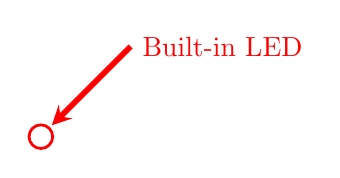
\begin{tikzpicture}
				\tikzset{
					lineScaled/.style={line width={2pt}},
					arrowStyle/.style={lineScaled, >=stealth, red},
					boxStyle/.style={line width={1pt}, red},
				}
				\ArduinoMkrWan{0.4}{270}{0}{0}{0}
				
				\draw[boxStyle] (-1.64, 1.175) circle (0.15cm);
				\draw[arrowStyle, <-] (-1.5, 1.32) -- ++(1, 1) node[right]{Built-in LED};
			\end{tikzpicture}
			\captionof{figure}{Integrierte LED auf dem Arduino MKR WAN 1310}
			\label{fig:builtInLED}
		\end{center}
		
	\end{enumerate}

